\chapter{Anwendungsmöglichkeiten der Blockchain/smarter Verträge}\label{chapter_anwendungsmöglichkeiten}
\section{Anwendungsmöglichkeiten}
\subsection{Dezentrale, autonome Organisationen (DAOs)}
\todo{Decentralized Autonomous Corporation - Daniel Larimer}
\todo{DAO - Vitalik Buterin}
\todo{Distributed Collaborative Organization - Joel Dietz}
\subsubsection{Begriffsbeschreibung}
Einer der wohl spannendsten Anwendungsfelder besteht in der Verwendung von Blockchain-Technologie um eine dezentrale, autonome Organisation (DAO) aufzubauen. Vitalik Buterin bemüht sich hierbei um eine Begriffserklärung, was eine DAO ist.

\begin{figure}[ht]
	\centering
	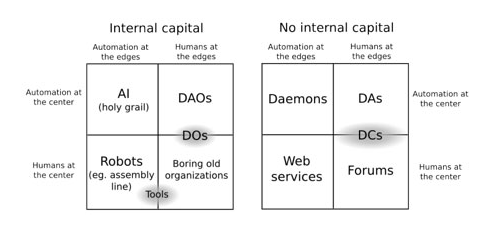
\includegraphics[scale=0.75]{grafiken/Abgrenzung_DAO.png}
	\caption{Verschiedene Unternehmensformen nach Art von Mensch und Maschinen-interaktion \cite{Buterin.2014c}}
	\label{dao_abgrenzung}
\end{figure}

Wie in Abbildung \ref{dao_abgrenzung} ersichtlich wird, unterteilt er verschiedene Organisationsarten zunächst danach, ob sie eigenes Kapital verwalten und dann danach, in welcher weise Mensch und Maschine miteinander interagieren. Automatisierung in der Mitte drückt aus, dass im Zentrum der Organisation Maschinen stehen mit denen interagiert wird. Automatisierung am Rand drückt aus, dass Maschinen mit dem Zentrum der Organisation interagieren. Gleiches gilt für Menschen im Zentrum und am Rand. Entsprechend ergeben sich acht Organisationsformen:
\begin{enumerate}
	\item Decentralized Applications (DAs) - Dezentralisierte Anwendungen, wie z.B. Peer-to-Peer Netzwerke wie Skype oder Bittorrent, in denen Menschen über ein dezentralisiertes Netzwerk direkt miteinander interagieren. Zu solchen Anwendungen ließe sich auch das frühe Internet zählen, bevor es hierarchisiert wurde.
	\item Foren - Menschen interagieren mit Menschen und bauen dadurch eine Organisation auf.
	\item Web Services - 
	\item Daemons - Beispielsweise Systemprogramme, die automatisch ausgeführt werden
	\item gewöhnliche Organisationen - Systeme werden zwar unterstützend genutzt, jedoch wird sie komplett von Menschen geführt
	\item Roboter - 
	\item DAOs - in der Mitte steht eine Anwendung, die autonom läuft, d.h. Grundfunktionen, wie z.B. Gehaltsströme würden auch ohne menschliche Interaktion funktionieren. Dezentral ist sie derart, dass ihr Programmcode nicht von einer zentralen Stelle verändert oder gelöscht werden kann. Menschliche Interaktion besteht in der Verwaltung der DAO, beispielweise ihrer Mitglieder oder dritter Parteien, die durch eine DAO bezahlt werden und dafür einen Profit erwirtschaften sollen.
	\item AI - Eine Organisation, die sich komplett selbst verwaltet
	
\end{enumerate}
\todo{Genauer beschreiben was eine DAO ist, durch zusammensetzen der Wörter dezentralisiert, autonom und organisation - Bitcoin als erste DAO oder DAC (Begrifflichkeiten klären - siehe https://www.youtube.com/watch?v=QG-CcbtwKKU\&list=PLjgfpSQFJTLpKmTGCG8FjvDFbfst6F-x5\&index=2 und https://blog.ethereum.org/2014/05/06/daos-dacs-das-and-more-an-incomplete-terminology-guide/)}
\footnote{http://cointelegraph.com/news/decentralized-autonomous-organizations-ethereum-sparks-up-googles-of-tomorrow} Einen starken medialen Anklang findet das Konzept von \ac{DAO}s. Sie stellen eine Art von Organisation auf der Blockchain dar, die ähnlich dem Crowdfounding von einer breiten Masse finanziert werden. Eine DAO verknüpft dabei jedoch die Vorteile des Crowdfounding und einer Aktiengesellschaft. Anstatt das Geld zu spenden, wird eine von der DAO verwaltete Währung - ein sogenannter Token - gekauft. Dieser Token repräsentiert einerseits einen gewissen Anteil an Stimmrechten, die Entscheidungen der DAO betreffen, sowie ein gewisser Anteil an Gewinnauszahlungen. Jeder Käufer von Tokens ist damit quasi ein Anteilseigner dieser Organisation.\\

\subsubsection{Rechtliche Grundlagen einer DAO}
Der rechtliche Status einer DAO ist bisher völlig ungeklärt. Da sie als Entität auf der Blockchain nicht in irgendeinem bestimmten Land ansässig ist, wird sie wohl für unbestimmte Zeit keinen Status als juristische Person erlangen. Dies führt zu zum Teil recht abenteuerlichen rechtlichen Konstrukten. Stephen Palley beschreibt in einem Blog-Beitrag den Status einer DAO aus der Perspektive Britischen Rechts. Laut ihm würde eine DAO einem \glqq General Partnership\grqq{} entsprechen. In dieser Form sind die Teilnehmer in einer DAO voll haftbar. Zusätzlich würde es vor Gericht ausreichen, einen Teilnehmer einer DAO zu identifizieren, dieser wäre dann verantwortlich dafür, eine Strafe gleichmäßig auf die Teilnehmer zu verteilen.

- Weltweit verteilt --> wem und wie werden steuern bezahlt?\\
- Wie kann sie angeklagt werden?\\
- Wer klagt sie an?\\

\section{Praxisbeispiele}
\subsection{Verknüpfung von IOT und Blockchain: slock.it}
\subsection{Hedging über digitales Gold: digix}
Gold kaufen über Blockchain
\subsection{Dezentralisierte Prognosemärkte: Augur}
\subsection{Coins mit gekoppelter Wertentwicklung: Bitshares}
\subsection{smart Property}
\begin{itemize}
	\item Tokens/eigene Währungen
\item Namecoins
\item Colored coins
\item Smart-Contract
\item Decentralized autonomous organizations DAOs
\item Smart properties
\item Token Systeme (Generierung einer eigenen Währung, die z.B. den Anspruch auf ein Wertpapier definiert (smart property)
\item Financial derivatives and Stable-Value Currencies (Generierung einer eigenen Währung, die einen fixen Wert, z.B. 1000USD hat. Wenn sich beide Parteien darauf einigen, 
\item Identity and Reputation Systems (Named coins, z.B. registrierung von Domain-Namen auf der blockchain
\item Decentralized File Storage (Benutzung von speicherplatz auf Basis von mikro-payments
\item Decentralized Autonomous Organizations
\item Savings wallets
\item Crop insurance
\item A decentralized data feed
\item Smart multisignature escrow
\item Cloud computing
\item Peer-to-peer gambling
\item Prediction markets
Augur
\item On-chain decentralized marketplace
\end{itemize}